\documentclass[a4paper, twocolumn]{article} %可加上 twocolumn 來變成雙欄格式
\usepackage{fontspec}   %加這個就可以設定字體
\usepackage{xeCJK}       %讓中英文字體分開設置
\usepackage{indentfirst}
\usepackage{listings}
\usepackage[newfloat]{minted}
\usepackage{float}
\usepackage{graphicx}
\usepackage{caption}
\usepackage{fancyhdr}
\usepackage{hyperref}
\usepackage{amsmath}
\usepackage{multirow}
\usepackage[dvipsnames]{xcolor}
\usepackage{graphicx}
\usepackage{tabularx}
\usepackage{booktabs}
\usepackage{caption}
\usepackage{subcaption}
\usepackage{pifont}
\usepackage{amssymb}
\usepackage[backend=biber]{biblatex}
\addbibresource{main.bib}


\usepackage{pdftexcmds}
\usepackage{catchfile}
\usepackage{ifluatex}
\usepackage{ifplatform}

\usepackage[breakable, listings, skins, minted]{tcolorbox}
\usepackage{etoolbox}
\setminted{fontsize=\footnotesize}
\renewtcblisting{minted}{%
    listing engine=minted,
    minted language=python,
    listing only,
    breakable,
    enhanced,
    minted options = {
        linenos, 
        breaklines=true, 
        breakbefore=., 
        % fontsize=\footnotesize, 
        numbersep=2mm
    },
    overlay={%
        \begin{tcbclipinterior}
            \fill[gray!25] (frame.south west) rectangle ([xshift=4mm]frame.north west);
        \end{tcbclipinterior}
    }   
}

\usepackage[
top=1.5cm,
bottom=0.75cm,
left=1.5cm,
right=1.5cm,
includehead,includefoot,
heightrounded, % to avoid spurious underfull messages
]{geometry} 

\newenvironment{code}{\captionsetup{type=listing}}{}
\SetupFloatingEnvironment{listing}{name=Code}


% set the title and name
\title{VRDL, 2026 Spring, HW1}
\author{112550011 李佑軒}
\date{\today}


% \setCJKmainfont{Noto Serif TC}
\setCJKmainfont{Microsoft JhengHei}


\ifwindows
\setmonofont[Mapping=tex-text]{Consolas}
\fi

\XeTeXlinebreaklocale "zh"             %這兩行一定要加，中文才能自動換行
\XeTeXlinebreakskip = 0pt plus 1pt     %這兩行一定要加，中文才能自動換行

\newcommand*{\dif}{\mathop{}\!\mathrm{d}}

\begin{document}
\maketitle % write the title, name and date

\section{Introduction}
In this assignment, we need to work on a multi-class classfication task involving 100 distinct object categories.
The dataset consist of approximately 21,024 traing/validation images and 2344 test images. 
The primary challenge is achieving high generalization performance with a small number of sample per category
while confining to the constraint that the model backbone must be ResNet-based architecture with fewer than 100 million parameters.

Our core stategy involves leveraging Transfer Learning by utilizing the backbone such as ResNet-50, ResNet-101 and ResNet-152
pre-trained on ImageNet-1K (V2 weights). To avoid overfitting, I tried many strategies to enhance model's capacity.
I implemented many stategies such as RandAugment, Mixup, and CutMix. Futhermore, I employed Test-Time Augmenation during inference to stablize predictions
and further boost accuracy, aiming to surpass the "strong-baseline" of 0.94.

\section{Method}
\subsection{Data Preprocessing and Augmenation}
To achieve high generalization on a 100-class dataset with limited samples, we implemented a sophisticated training 
"recipe" combining spatial, pixel-level, and label-based regularization.
These techniques collectively prevent the ResNet-based backbone from memorizing training instances and
instead force it to learn robust, discriminative features.
\begin{itemize}
    \item \textbf{Random Resized Crop and Random Horizontal Flip}: We apply random resized (scale (0.08, 1.0)) cropping to 224x224 pixels and random horizontal flipping with a probability of 0.5 to further enhance spatial diversity. This forces the model to recognize objects from extremely small patches (as little as 8\% of the original image). This is crucial for 100-category classification where discriminative features might only reside in localized regions (e.g., the beak of a bird or the texture of a leaf). 
    \item \textbf{RandAugment} \cite{RandAugment_pulished, RandAugment_pytorch}: We apply RandAugment with $N=2$ (the number of sequential transformations applied to each image) and $M=9$ (controls the intensity of transformations) to introduce diverse transformations. By randomly applying diverse transforms, we significantly expand the data distribution, ensuring the model is invariant to lighting conditions and minor geometric distortions.
    \item \textbf{Normalization}: We normalize the images using the mean and standard deviation of the ImageNet dataset to ensure that the input data is on a similar scale as the pre-trained ResNet backbones, facilitating better convergence during fine-tuning.
    \item \textbf{Mixup and Cutmix} \cite{mixup_pulished, cutmix_pulished, MixUp_CutMix_pytorch}: To further regularize the decision boundaries, we integrated Mixup and CutMix. Blends two images and their labels linearly using a coefficient $\lambda$ derived from a Beta distribution ($\alpha=1.0$). CutMix: Replaces a random rectangular region of one image with a patch from another, with labels mixed proportionally to the area. These methods transition the model from "hard" one-hot labels to "soft" probability distributions. Consequently, Training Accuracy may appear lower (often staying between 70\%-80\% during training) because the model is solving a much harder task: identifying multiple overlapping objects. However, this "harder" training task translates to significantly higher Validation Accuracy and better generalization to the test set.
    \item \textbf{label smoothing} \cite{label_smoothing_pulished}: We apply label smoothing with a factor of small number 0.1 to prevent the model from becoming overconfident in its predictions. This technique encourages the model to assign some probability mass to incorrect classes, which can improve generalization and reduce overfitting, especially in a multi-class setting with many categories.
\end{itemize} 

\subsection{Model Architecture and Training}
We utilize ResNet-50, ResNet-101, and ResNet-152 backbones, which are all well within the 100M parameter limit and pre-trained on ImageNet-1K (V2 weights) for transfer learning. And training stategy and hyperparameters are as follows:
\begin{itemize}
    \item \textbf{Backbone Modification}: We replace the final fully connected layer of the ResNet backbones with a new layer that outputs 100 classes, corresponding to our dataset. This allows us to leverage the rich feature representations learned from ImageNet while adapting to our specific classification task.
    \item \textbf{Dropout}: We add a dropout layer with a rate of 0.5 before the final classification layer to further prevent overfitting by randomly deactivating neurons during training. And activate all the dropout layers during inference to stablize the predictions.
    \item \textbf{Optimizer}: We used AdamW with a weight decay of $5 \times 10^{-4}$ to regulate weight magnitudes.
    \item \textbf{Learning Rate Scheduler}: A Cosine Annealing scheduler was employed over 100, 200 epochs, preceded by a 5, 10-epoch Warmup phase where the backbone was frozen to stabilize the new classification head.
    \item \textbf{Loss Function}: Cross Entropy Loss with Label Smoothing (0.1) was used to prevent the model from becoming overly confident in its predictions.
\end{itemize}

\subsection{Inference and Test-Time Augmentation}
To maximize test accuracy, we implemented a 7-view Test-Time Augmentation (TTA) strategy. For each test image, we generated seven versions: the original center-cropped image, four corner crops, horizontal flips and small rotations. The final prediction was determined by Soft Voting, which averages the softmax probability distributions across all seven views to produce a more reliable class assignment.


\section{Results}

In this section, we present the final performance of our image classification system. Our best-performing submission was achieved through an ensemble of three ResNet architectures, integrated with Test-Time Augmentation (TTA) and majority voting.

\subsection{Final Training Configuration}
The following settings represent the optimized configuration used to produce our final results. To ensure consistency and robustness, the core hyperparameters were shared across all three backbone models:

\begin{itemize}
    \item \textbf{Model Backbones}: An ensemble of ResNet-50, ResNet-101, and ResNet-152, all utilizing ImageNet-1K V2 pre-trained weights. And only use one fc layer as the classification head for all three backbones to reduce the risk of overfitting.
    \item \textbf{Data Augmentation \& Regularization}:
    \begin{itemize}
        \item \textbf{Augmentation}: RandResizedCrop, RandAugment, Mixup ($\alpha=1.0$), and CutMix ($\alpha=1.0$).
        \item \textbf{Regularization}: Weight Decay($5 \times 10^{-4}$), Label Smoothing (0.1) and Dropout (0.5).
        \item \textbf{Spatial Invariance}: RandomResizedCrop with a scale of (0.08, 1.0).
    \end{itemize}
    \item \textbf{Optimization}:
    \begin{itemize}
        \item \textbf{Optimizer}: AdamW with a weight decay of $5 \times 10^{-4}$.
        \item \textbf{Learning Rate}: $1 \times 10^{-3}$ (FC head) and $1 \times 10^{-4}$ (Backbone).
        \item \textbf{Scheduler}: Cosine Annealing.
    \end{itemize}
    \item \textbf{Other Training Settings}:
    \begin{itemize}
        \item \textbf{Batch Size}: 64
        \item \textbf{Epochs}: 100 for ResNet-50 and ResNet-101, 200 for ResNet-152. Since ResNet-152 has a higher capacity, it benefits from a longer training epochs.
        \item \textbf{Backbone Freezing}: During the Warmup phase, the backbone was frozen to allow the new classification head to stabilize before fine-tuning the entire network. 5 epochs for ResNet-50 and ResNet-101, 10 epochs for ResNet-152.
    \end{itemize}
    \item \textbf{Inference Strategy}: 7-view TTA (including center/corner crops, horizontal flips, and small rotations) combined with Soft Voting (addition of output probabilities) before the final Majority Vote ensemble.
\end{itemize}

\subsection{Final Performance}
By integrating the aforementioned strategies, our three models all achieved strong validation performanced (all above 90\% acc). Also, three models beat strong baseline of 94\% on thier own. The final ensemble, which combined the predictions of all three models using majority voting, achieved a test accuracy of 96\% on the public leaderboard, surpassing our initial target and demonstrating the effectiveness of our training and inference strategies.
\begin{table}[h]
\centering
\caption{Best Validation Accuracy achieved during the training phase.}
\label{tab:val_acc}
\begin{tabular}{@{}lc@{}}
\toprule
\textbf{Model Backbone} & \textbf{Best Validation Accuracy (\%)} \\ \midrule
ResNet-50               & 90.33\%                    \\
ResNet-101              & 90\%                    \\
ResNet-152              & \textbf{91.67}\%                    \\ \bottomrule
\end{tabular}
\end{table}

% --- Table 2: Test Accuracy & Ensemble Result ---
\begin{table}[h]
\centering
\caption{Comparison of individual model test accuracy and final ensemble performance. (test accuracy is obtained from public leaderboard)}
\label{tab:test_acc}
\begin{tabular}{@{}lc@{}}
\toprule
\textbf{Submission / Model} & \textbf{Test Accuracy (\%)} \\ \midrule
ResNet-50 (Single + TTA)    & 95\%        \\
ResNet-101 (Single + TTA)   & 95\%        \\
ResNet-152 (Single + TTA)   & 95\%        \\ \midrule
\textbf{Ensemble (Majority Vote)} & \textbf{96\%}            \\ \bottomrule
\end{tabular}
\end{table}

The training and validation curves for our primary models are illustrated in Figure \ref{fig:training_curves}, showing stable convergence and effective regularization throughout the training process.


\begin{figure}[h]
    \centering
    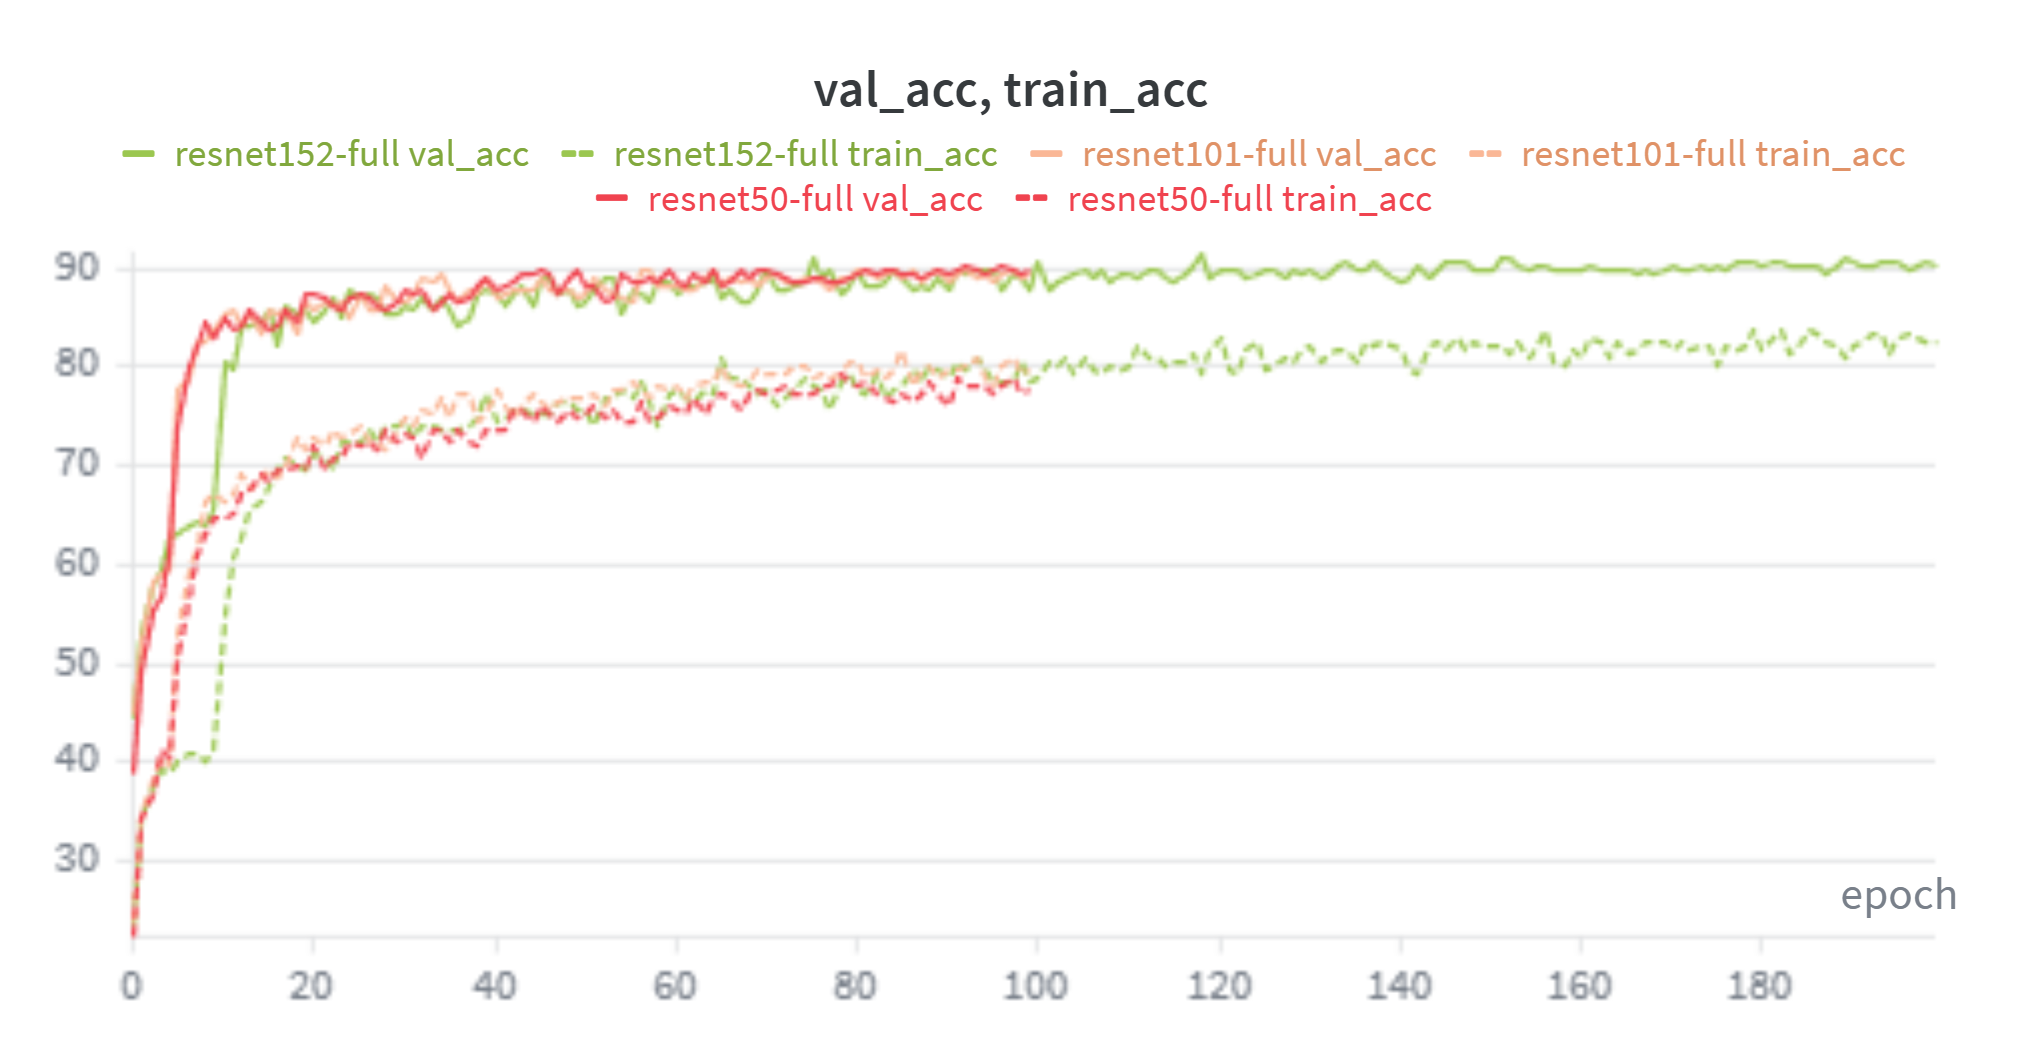
\includegraphics[width=0.95\linewidth]{figures/train_result.png}
    \caption{Training and Validation Accuracy/Loss curves.}
    \label{fig:training_curves}
\end{figure}


\section{Additional Experiments}
To further understand the contribution of each component in our training "recipe," we conducted some ablation studies 
on the ResNet-50 and ResNet-152 backbone. Note that since validation data is small (only contain 300 samples), the validation result will contain high variance. But we can still observe the general trend of the training and validation curves to understand the impact of each component.
\subsection{Impact of RandAugment}
We conducted a experiment show in Figure \ref{fig:without_aug} since I thought that without the diverse pixel-level and geometric transformations 
provided by RandAugment, the model would easily overfit to 
the limited training samples, failing to learn generalized features.
\begin{figure}[h]
    \centering
    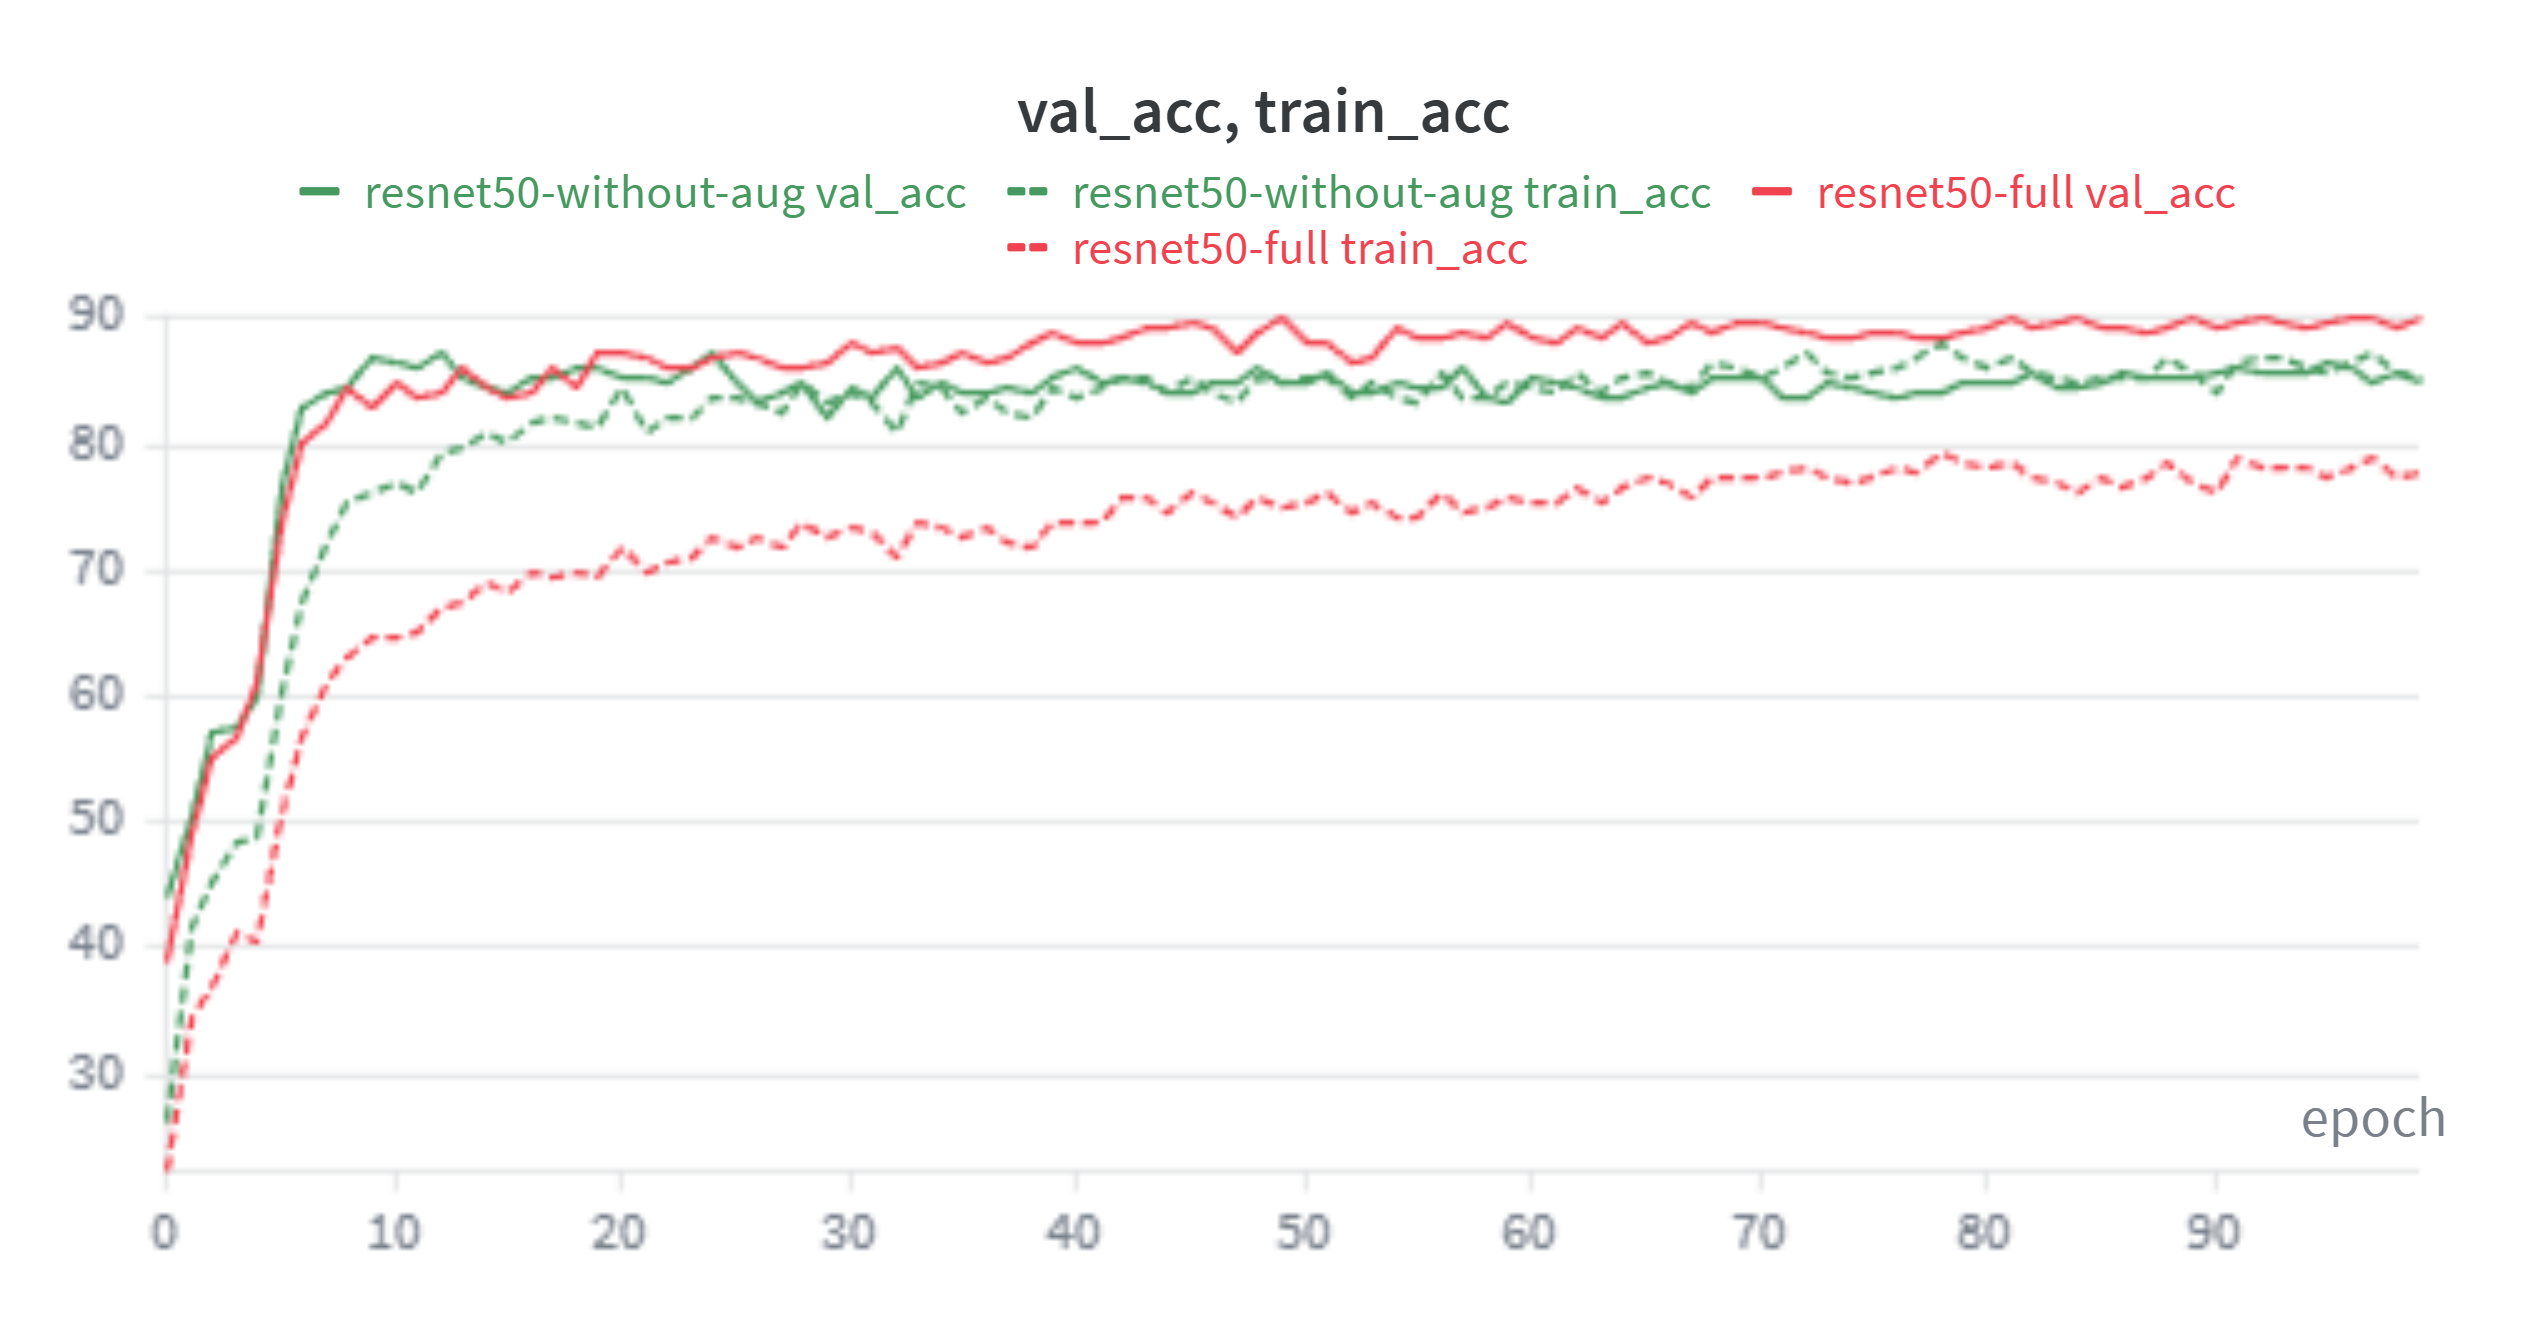
\includegraphics[width=0.95\linewidth]{figures/without_aug.png}
    \caption{As illustrated in the training curves, the model without RandAugment (green dashed line) reached a high 
    training accuracy (~85\%) very rapidly, yet its validation accuracy (green solid line) reach at around 87\% rapidly, then drop to around 85\% and stuck on the long run. 
    In contrast, the full model (red lines) showed a lower training accuracy due to the increased task difficulty but achieved 
    a higher and more stable validation accuracy (around 90\%). This confirms that RandAugment is crucial for bridging the generalization gap by preventing the model from "memorizing" specific image patterns.}
    \label{fig:without_aug}
\end{figure}

\subsection{Impact of Mixup and CutMix}
We conducted an experiment shown in Figure \ref{fig:without_mix} since we thought that without Mixup and CutMix, the validation accuracy would drop, and the model would be more prone to overfit the training data.

\begin{figure}[h]
    \centering
    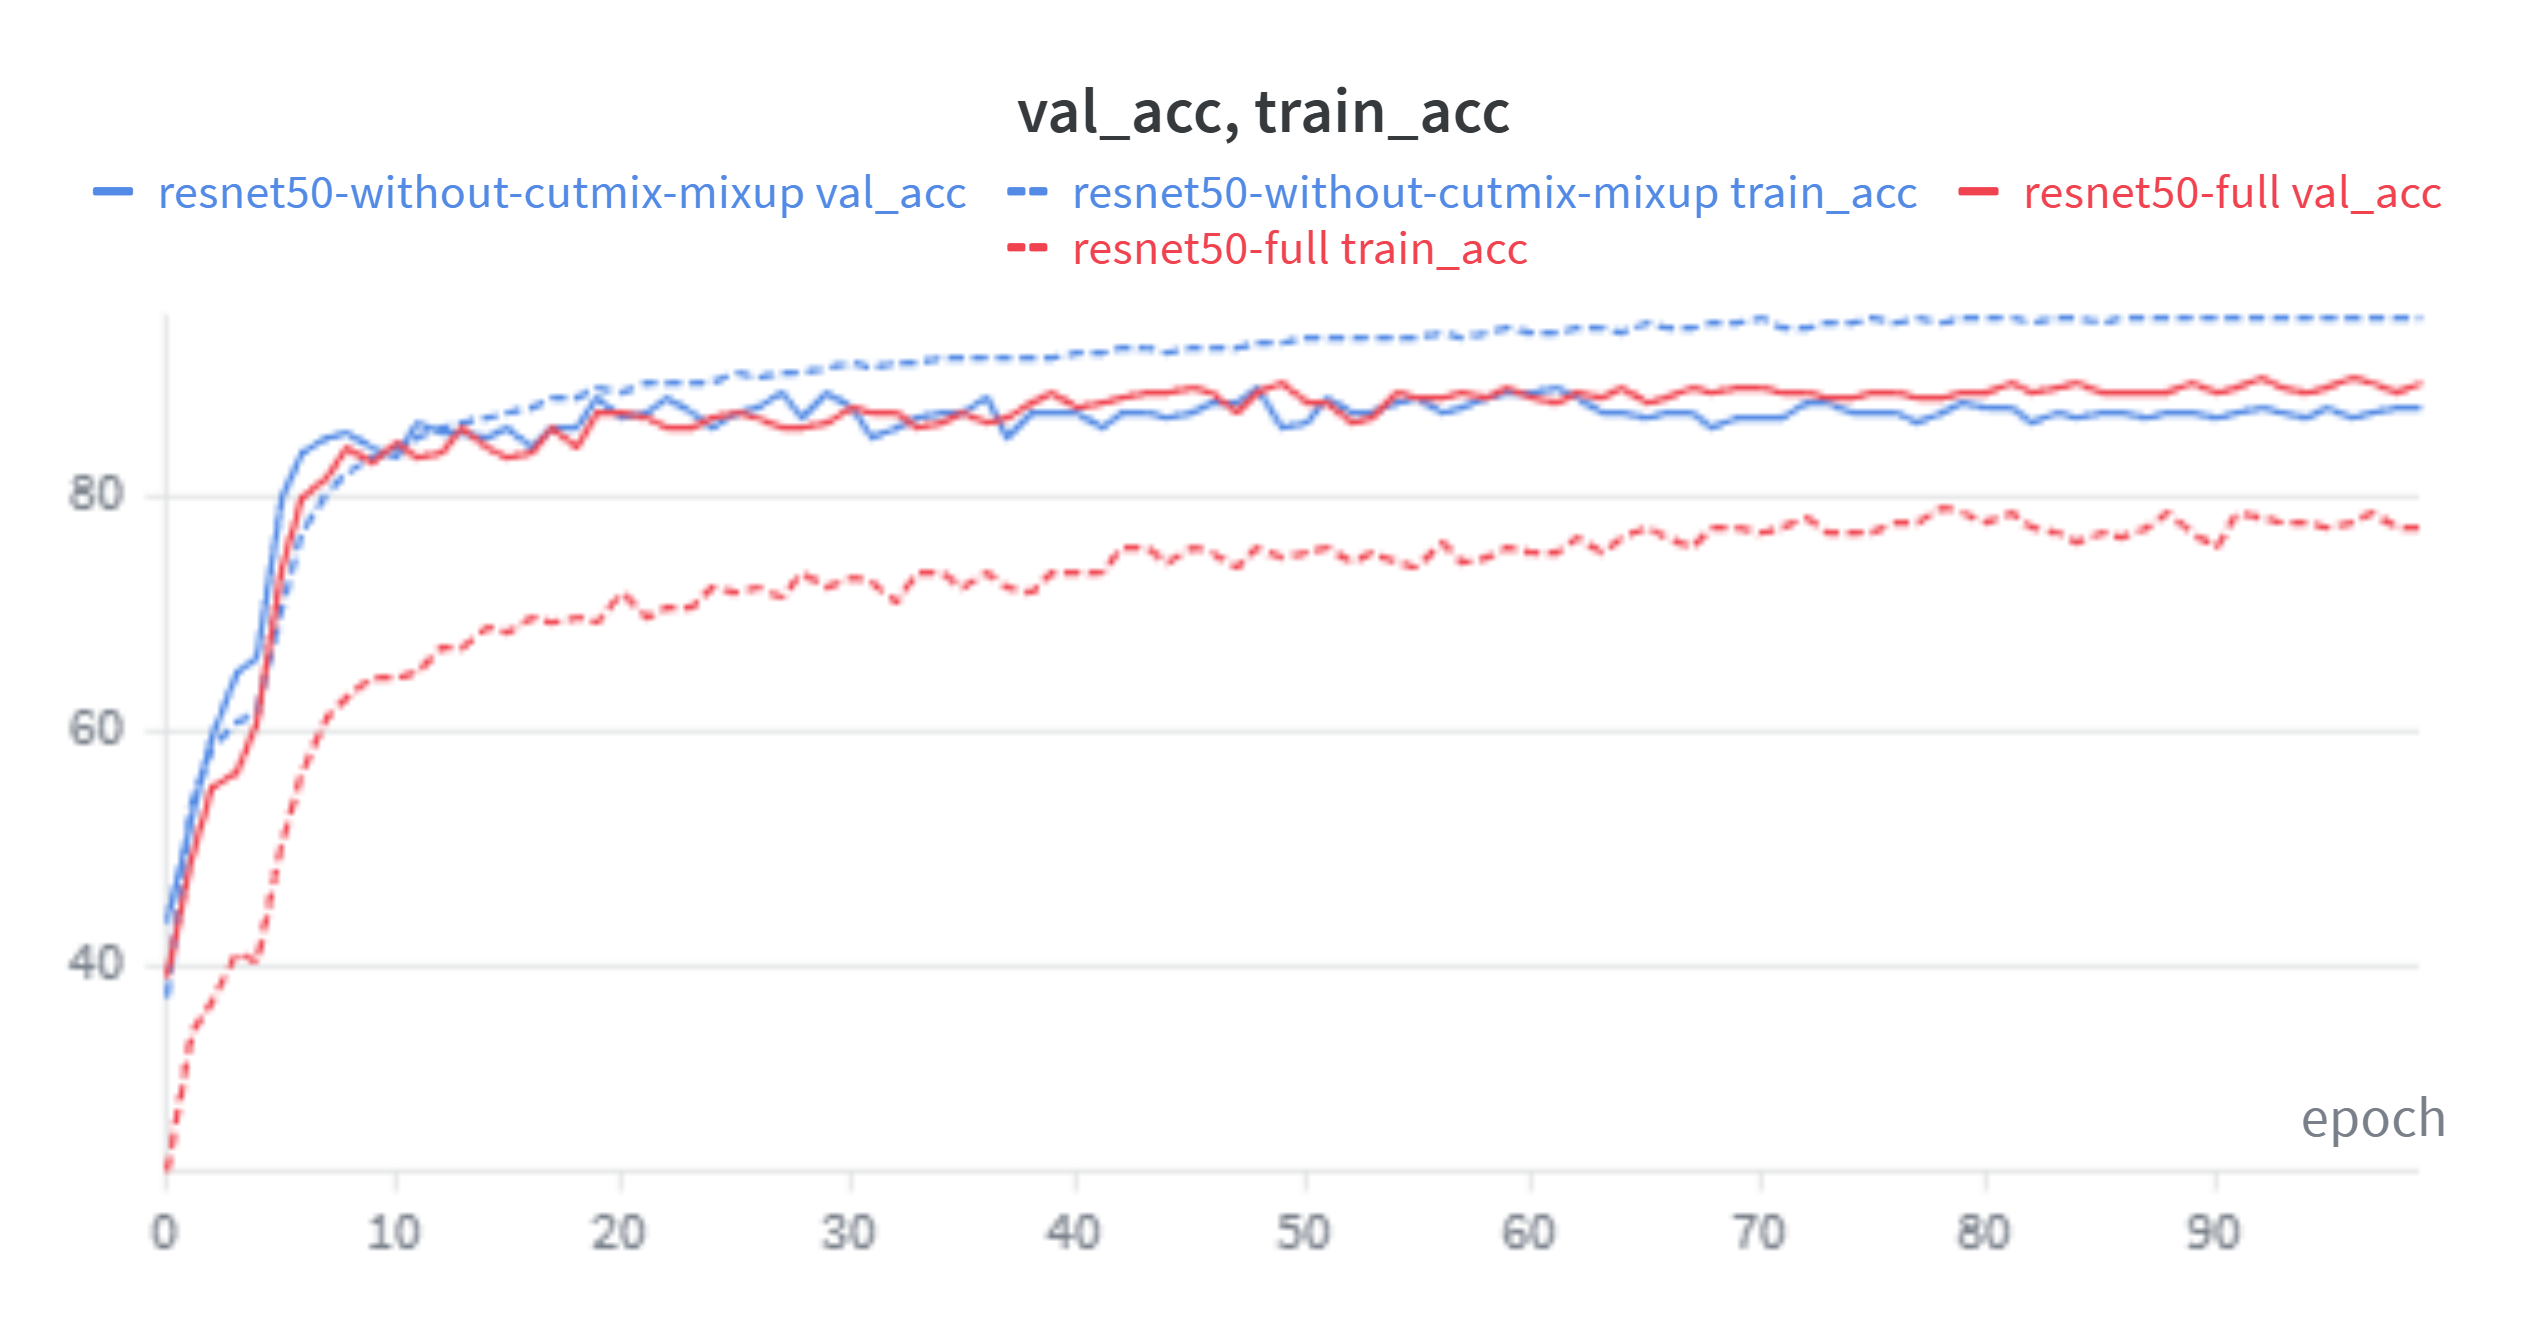
\includegraphics[width=0.95\linewidth]{figures/without_mix.png}
    \caption{The results (blue lines) clearly demonstrate the danger of "label over-confidence." Without Mixup/CutMix, 
    the training accuracy (blue dashed line) shot up to nearly 99\% very fast, indicating severe overfitting. 
    While its initial validation speed was fast, it was eventually surpassed by the full model (red solid line). 
    The "full" model exhibits a much smaller gap between training and validation accuracy. 
    This implies that the convex combination of images and labels serves as a powerful regularizer that encourages
    the model to learn smoother decision boundaries, which is important for achieving high performance in a 100-class classification task.
    }
    \label{fig:without_mix}
\end{figure}

\subsection{Impact of weight decay}
The experiment in Figure \ref{fig:without_wd} is the expriment without weight decay. We assume that without weight decay, the model weight might grow excessively, leading to overfitting. We compared the training dynamics of ResNet-152 with and without Weight Decay (WD) ($\lambda = 5 \times 10^{-4}$).

\begin{figure}[h]
    \centering
    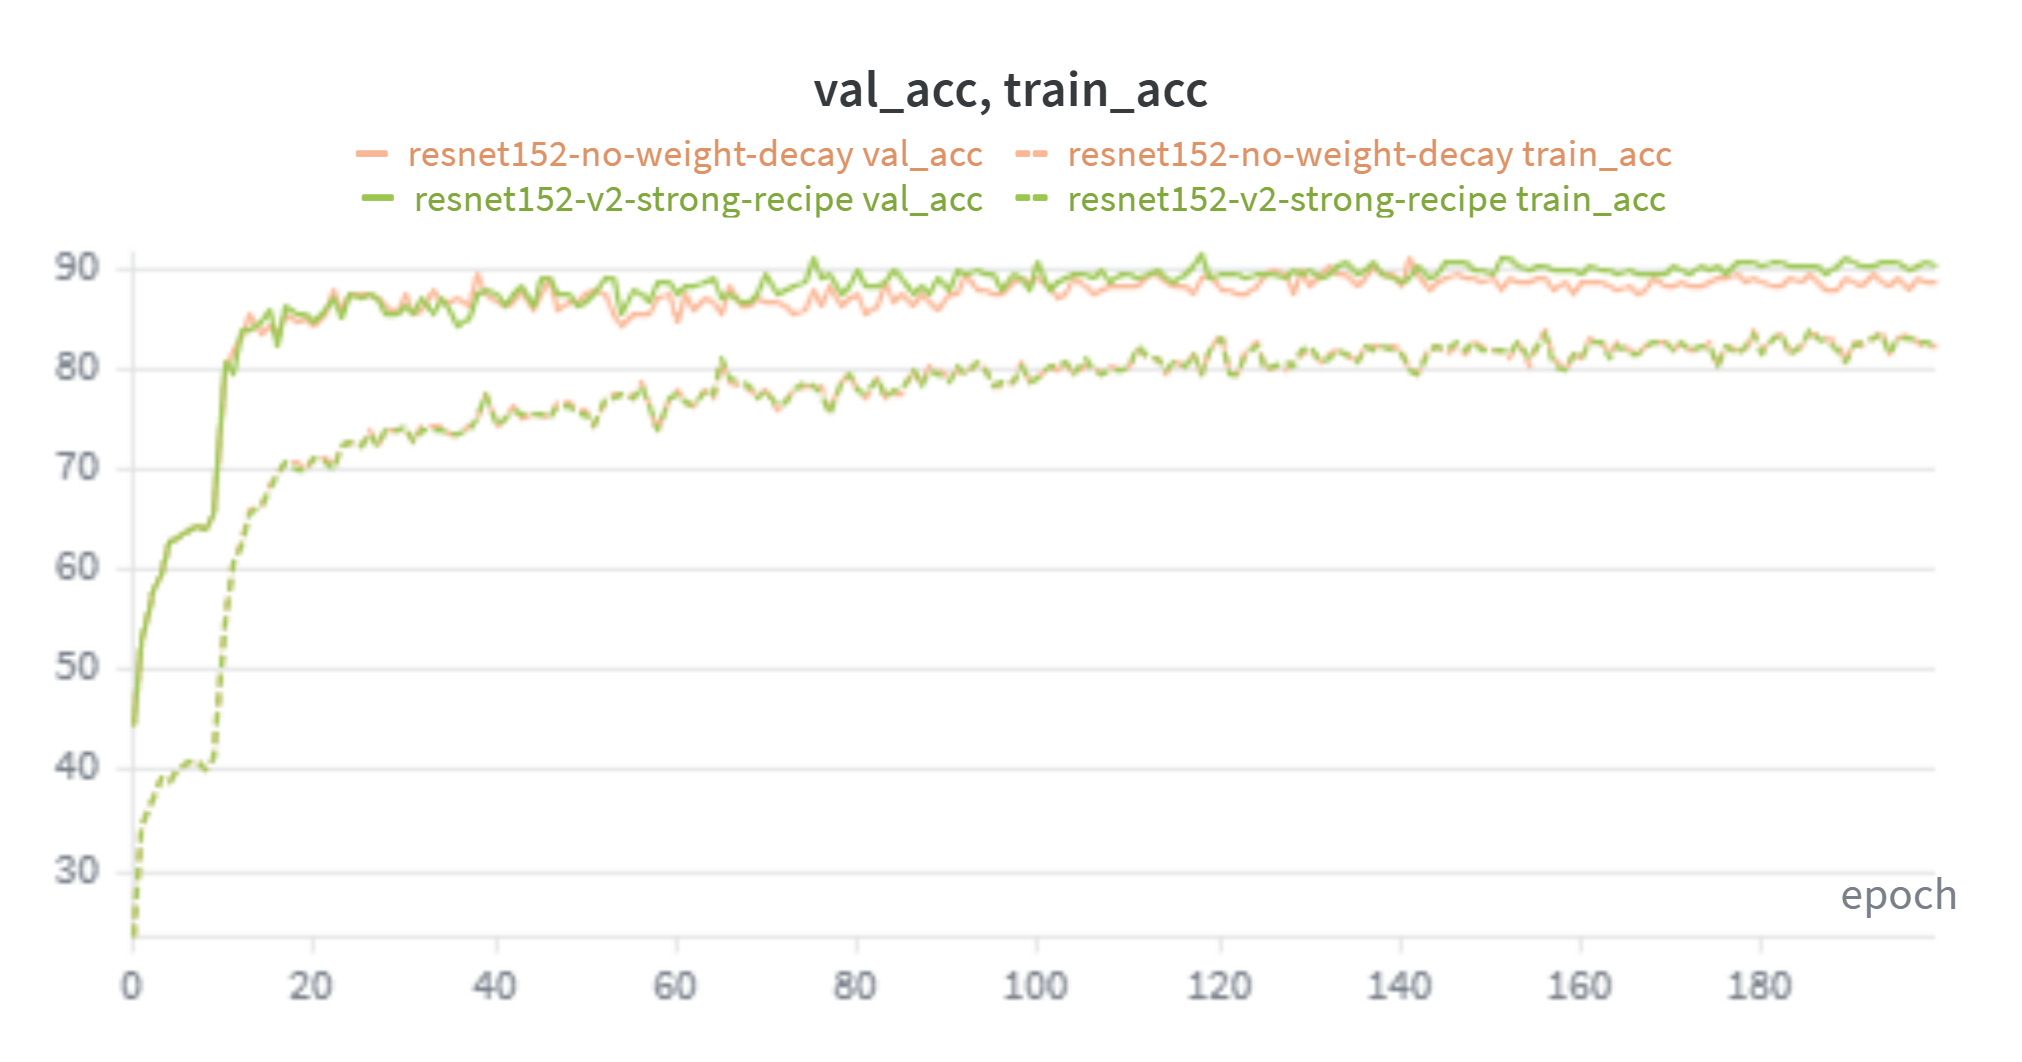
\includegraphics[width=0.95\linewidth]{figures/no_wd.png}
    \caption{
        Since we employed aggressive techniques like Mixup, CutMix, and RandAugment, the regularization effect provided by these data-level augmentations is significantly more impactful than the $L_2$ penalty from Weight Decay. The model is primarily struggling to fit the complex, augmented samples, making the subtle influence of WD less visible on the training curve.
        While the training curves are similar, the validation accuracy (solid lines) reveals the true benefit of Weight Decay. The model trained with WD (green solid line) consistently maintains a slight margin (approx. 1.0\%-2.0\%) over the version without it (orange solid line) in the later stages of training.
    }
    \label{fig:without_wd}
\end{figure}
\printbibliography % to print the bibliography
\end{document}